%% 
%% Copyright 2007, 2008, 2009 Elsevier Ltd
%% 
%% This file is part of the 'Elsarticle Bundle'.
%% ---------------------------------------------
%% 
%% It may be distributed under the conditions of the LaTeX Project Public
%% License, either version 1.2 of this license or (at your option) any
%% later version.  The latest version of this license is in
%%    http://www.latex-project.org/lppl.txt
%% and version 1.2 or later is part of all distributions of LaTeX
%% version 1999/12/01 or later.
%% 
%% The list of all files belonging to the 'Elsarticle Bundle' is
%% given in the file `manifest.txt'.
%% 

%% Template article for Elsevier's document class `elsarticle'
%% with numbered style bibliographic references
%% SP 2008/03/01

\documentclass[preprint,12pt]{elsarticle}

%% Use the option review to obtain double line spacing
%% \documentclass[authoryear,preprint,review,12pt]{elsarticle}

%% Use the options 1p,twocolumn; 3p; 3p,twocolumn; 5p; or 5p,twocolumn
%% for a journal layout:
%% \documentclass[final,1p,times]{elsarticle}
%% \documentclass[final,1p,times,twocolumn]{elsarticle}
%% \documentclass[final,3p,times]{elsarticle}
%% \documentclass[final,3p,times,twocolumn]{elsarticle}
%% \documentclass[final,5p,times]{elsarticle}
%% \documentclass[final,5p,times,twocolumn]{elsarticle}

%% For including figures, graphicx.sty has been loaded in
%% elsarticle.cls. If you prefer to use the old commands
%% please give \usepackage{epsfig}

\usepackage{epsfig}
\usepackage{caption}

%%%%%% For subfigures on multiple pages
 
\usepackage{caption}
\makeatletter\def\CT{\def\@captype{figure}}\makeatother

%%%%%%

%% The amssymb package provides various useful mathematical symbols
\usepackage{amssymb}
%% The amsthm package provides extended theorem environments
%% \usepackage{amsthm}

%% The lineno packages adds line numbers. Start line numbering with
%% \begin{linenumbers}, end it with \end{linenumbers}. Or switch it on
%% for the whole article with \linenumbers.
\usepackage{lineno}

%\usepackage{epstopdf}

\usepackage[caption=false]{subfig} 
\usepackage{color}

\journal{Physica A}

\begin{document}

\begin{frontmatter}

%% Title, authors and addresses

%% use the tnoteref command within \title for footnotes;
%% use the tnotetext command for theassociated footnote;
%% use the fnref command within \author or \address for footnotes;
%% use the fntext command for theassociated footnote;
%% use the corref command within \author for corresponding author footnotes;
%% use the cortext command for theassociated footnote;
%% use the ead command for the email address,
%% and the form \ead[url] for the home page:
%% \title{Title\tnoteref{label1}}
%% \tnotetext[label1]{}
%% \author{Name\corref{cor1}\fnref{label2}}
%% \ead{email address}
%% \ead[url]{home page}
%% \fntext[label2]{}
%% \cortext[cor1]{}
%% \address{Address\fnref{label3}}
%% \fntext[label3]{}

\title{Room evacuation through two contiguous exits}

%% use optional labels to link authors explicitly to addresses:
\author[label1]{I.M.~Sticco}
\author[label3]{G.A.~Frank}
\author[label1]{S.~Cerrotta}
\author[label1,label2]{C.O.~Dorso}
\address[label1]{Departamento de F\'\i sica, Facultad de Ciencias 
Exactas y Naturales, Universidad de Buenos Aires, Pabell\'on I, Ciudad 
Universitaria, 1428 Buenos Aires, Argentina.}
\address[label2]{Instituto de F\'\i sica de Buenos Aires, Pabell\'on I, Ciudad 
Universitaria, 1428 Buenos Aires, Argentina.}
\address[label3]{ Unidad de Investigaci\'on y Desarrollo de las 
Ingenier\'\i as, Universidad Tecnol\'ogica Nacional, Facultad Regional Buenos 
Aires, Av. Medrano 951, 1179 Buenos Aires, Argentina.}

%%\author{}

%%\address{}

\begin{abstract}
%% Text of abstract
Current regulations demand that at least two exits should be available 
for a safe evacuation during a panic situation. The second exit is  
expected to reduce the overall clogging, and  consequently, improve the 
evacuation time. However, rooms having contiguous doors not always reduce the 
leaving time as expected. We investigated the relation between the door's 
separation and the evacuation performance. We found that there exists a 
separation distance range that does not really improve the evacuation time, or 
it can even worsen the process performance. To our knowledge, no attention has 
been given to this issue in the literature. This work reports how the 
pedestrian's dynamics differ when the separation distance between two exit doors 
changes and how this affects the overall performance.
\end{abstract}

\begin{keyword}
%% keywords here, in the form: keyword \sep keyword

Panic evacuation \sep Social force model \sep Clogging delay

%% PACS codes here, in the form: \PACS code \sep code

\PACS 45.70.Vn \sep 89.65.Lm

%% MSC codes here, in the form: \MSC code \sep code
%% or \MSC[2008] code \sep code (2000 is the default)

\end{keyword}

\end{frontmatter}

\linenumbers

\section{\label{introduction}Introduction}

The practice of providing two doors for emergency evacuation can be traced back 
to the last Qing dynasty in China (1644-1911 AD). A mandatory regulation 
established that large buildings had to provide two fire exits \cite{cheng}. 
This kind of regulations upgraded to current standard codes with detailed  
specifications on the exits position, widths and separations \cite{OSHA,FLO}. \\


Current regulations claim that the minimum door width should be 0.813~m while 
the maximum door-leaf should not exceed 1.219~m \cite{FLO,FLO2}. If more than 
two doors are required, the distance between two of them must be at least 
one-half or one-third of the room diagonal distance. But, no special 
requirements apply to the rest of the doors.  \\

The rulings leave some space for placing the extra openings (\emph{i.e.} those 
above two exits) at an arbitrary separation distance. Thus, it is possible to 
place a couple of doors on the same side of the room at any distance. The 
special case of two contiguous doors has been examined throughout the 
literature \cite{kirchner1,perez1,daoliang1,huanhuan1}.  \\

Kirchner and Schadschneider studied the pedestrians evacuation process through 
two contiguous doors using a cellular automaton model \cite{kirchner1}. The 
agents were able to leave the room under increasing panic situations for 
behavioural patterns varying from individualistic pedestrians to strongly 
coupled pedestrians moving like a \emph{herd}. The evacuation time was found 
to be independent of the separation distance between doors for the 
individualistic pedestrians in a panic situation. But if the pedestrians were 
allowed to move like a herd, an increasing evacuation time for small separation 
lengths (less than 10 individuals size) was reported. \\

The above conclusions are not in complete agreement with the investigation 
acknowledged in Ref.~\cite{perez1}. The authors assert that the total number of 
pedestrians leaving the room per unit time slows-down for separation 
distances (between doors) smaller than four door widths \cite{perez1}. This 
slow-down is identified as a disruptive interference effect due to pedestrians 
crossing in each other's path.  For the particular case analyzed in this work,  
the threshold of four door widths ($4\,d_w$) corresponds to the distance 
separation necessary to distinguish two independent groups of pedestrians, each 
one surrounding the nearest door. \\

Researchers called the attention on the fact that no matter how separated 
the two contiguous doors are placed, the overall performance does not improve 
twice with respect to a single exit (of the same total width). This 
effect is attributed to some sort of pedestrian interference  \cite{perez1}. 
\\

Although the above results were obtained for very narrow doors (\emph{i.e.} 
single individual width), further investigation showed that they also apply 
to doors allowing two simultaneous leaving pedestrians. However, this does 
not hold for a room with a single door \cite{daoliang1}. In this case, it is 
true that the mean flux of evacuating people increases with an increasing door 
width, but the ratio flux per door width decreases \cite{Dorso1}.   \\

It was observed in Ref.~\cite{kirchner1,daoliang1} that the two contiguous 
doors should not be placed near the wall corners, since the side walls affect 
negatively the evacuation efficiency. No further explanation was given on this 
phenomenon, although the authors concluded this may cause a worsening in the 
evacuation performance for large separation distances between doors.  \\


A recent investigation (Ref.~\cite{huanhuan1}) on evacuation processes of 
cellular automata suggests that five distances should be taken into account 
when studying the evacuation performance: the total width of the openings (that 
is, adding the widths of each door), the doors separation distance, the width 
difference between the two doors, and the distance to the nearest corner.   \\

From the results shown in Ref.~\cite{huanhuan1}, the evacuation time depends on 
the total width of the openings (if both doors have the same width). But, for 
a fixed total width of the opening, it appears that the optimal location of the 
exits depends on the doors separation distance. \\

Our investigation focuses on symmetric configurations with equally sized 
doors. At variance to the above mentioned literature, we examine the evacuation 
dynamics by means of the Social Force Model (SFM). An overview of this model 
can be found in Section \ref{background}. \\

In Section \ref{simulations} we describe the specific settings for the 
evacuation processes. The measurement conditions for the simulations can also 
be found there. \\

In Sections \ref{faster_is_slower} to \ref{null_gap_patterns} the single door 
configuration is revisited. Its purpose is to make easier the understanding of 
the two-doors configuration for very small separation distances $d_g$. \\

In Section \ref{door_seperation} we examine the case of two separated doors. 
We explore the effect of increasing the separation distance $d_g$ until the 
clogging areas close to each door become almost independent. \\

Section \ref{conclusions} resumes the pedestrians behavioural patterns, and its 
consequences on the evacuation performance, for the different door 
separation scenarios. \\  




\section{\label{background}Background}

\subsection{The Social Force Model}

The ``social force model'' (SFM) deals with the pedestrians behavioural 
pattern in a crowded environment. The basic model states that the 
pedestrians motion is controlled by three kind of forces: the ``desire force'', 
the ``social force'' and the ``granular force''. The three are very different in 
 nature, but enter into an equation of motion as follows  \\ 


\begin{equation}
m_i\,\displaystyle\frac{d\mathbf{v}^{(i)}}{dt}(t)=\mathbf{f}_d^{(i)}
(t)+\displaystyle\sum_{j}\displaystyle\mathbf{f}_s^{(ij)}(t)+\displaystyle\sum_{
j}\mathbf{f}_g^{(ij)}(t)\label{eqn_1}
\end{equation}

\noindent where $m_i$ is the mass of the pedestrian $i$, and $\mathbf{v}_i$ is 
its corresponding velocity. The subscript $j$ represents all other pedestrians 
(excluding $i$) and the walls. $\mathbf{f}_d$, $\mathbf{f}_s$ and 
$\mathbf{f}_g$ are the desire force, the social force and the granular force, 
respectively. See Refs.~\cite{Helbing1,Dorso1,Dorso2,Dorso3,Dorso4} for 
details.\\

The desire force reflects the pedestrian's own desire to go to a specific 
place \cite{Helbing1}. He (she) needs to accelerate (decelerate) from his (her) 
current velocity, in order to achieve his (her) own willings. As he (she) 
reaches the velocity that makes him (her) feel comfortable, no further 
acceleration (deceleration) is required. This velocity is the ``desired 
velocity'' of the pedestrian $\mathbf{v}_d(t)$. The expression for 
$\mathbf{f}_d$ in Eq.~(\ref{eqn_2}) handles this issue.  \\


\begin{equation}
\left\{\begin{array}{lcl}
        \mathbf{f}_d^ {(i)}(t) & = & m_i\,\displaystyle\frac{\mathbf{v}_d^
{(i)}(t)-\mathbf{v}_i(t)}{\tau} \\
        & & \\
\mathbf{f}_s^{(ij)} & = & A_i\,e^{(r_{ij}-d_{ij})/B_i}\mathbf{n}_{ij}\\
        & & \\
\mathbf{f}_g^{(ij)} &= &\kappa\,g(r_{ij}-d_{ij})\,\Delta
\mathbf{v}_{ij}\cdot\mathbf{t}_{ij} \\
       \end{array}\right.\label{eqn_2}
\end{equation}

$\tau$ means a relaxation time. Further details on each parameter can be found 
in Refs.~\cite{Helbing1,Dorso1,Dorso2,Dorso3,Dorso4}.\\

Notice that the desired velocity $\mathbf{v}_d$ has magnitude $v_d$ and points 
to the desired place at the direction $\hat{\mathbf{e}}_d$. Thus, $v_d$ 
represents his (her) state of anxiety, white $\hat{\mathbf{e}}_d$ indicates the 
place where he (she) is willing to go. We assume, for simplicity, that 
$v_d$ remains constant during an evacuation process, but $\hat{\mathbf{e}}_d$ 
changes according to the current position of the pedestrian.   \\

The social force $\mathbf{f}_s$ corresponds to the tendency of each individual 
to keep some space between him and other pedestrians, or, between him and the 
walls \cite{Helbing4}. The $\mathbf{f}_s$ expressed in Eq.~(\ref{eqn_2}) 
depends on the inter-pedestrian distance $d_{ij}$. The magnitude 
$r_{ij}=r_i+r_j$ is the sum of the pedestrian's radius, while $A_i$ and $B_i$ 
are two fixed parameters ($r_j=0$ for the interaction with the wall). Thus, 
$\mathbf{f}_s$ is a repulsive monotonic force that resembles the pedestrian 
feelings for preserving his (her) \textit{private sphere} 
\cite{Helbing1,Helbing4}. \\

The granular force $\mathbf{f}_g$ appearing in Eq.~(\ref{eqn_1}) represents the 
sliding friction between contacting people (or between people  and walls). Its 
expression can be seen also in Eq.~(\ref{eqn_2}). It is assumed to be a linear 
function of the relative (tangential) velocities $\Delta
\mathbf{v}_{ij}\cdot\mathbf{t}_{ij}$ of the contacting individuals. The 
function $g(r_{ij}-d_{ij})$ returns the argument value if $r_{ij}>d_{ij}$, 
while $\kappa$ is a fixed parameter (see 
Refs.~\cite{Helbing1,Dorso1,Dorso2,Dorso3,Dorso4}).\\

{\color{red} One of the most remarkable phenomena attained by this model is the ``faster is slower'' effect. It states that the higher the desired velocity, the higher the evacuation time~\cite{Helbing1}. Experimental data has achieved this effect, while the pressure of the bulk raises as a relevant magnitude in the worsening of the evacuation time. Experiments also show that the bulk pressure is a function of the number  of people and the maximum group speed. The latter is associated to the desired velocity in the Social Force Model (see Ref.~\cite{Pastor}).}  
 


\subsection{\label{human}Clustering structures}

The time delays during an evacuation process are related to clustering people 
as explained in Refs.~\cite{Dorso1,Dorso2}. Groups of pedestrians can 
be defined as the set of individuals that for any member of the group (say, 
$i$) there exists at least another member belonging to the same group ($j$) 
in contact with the former. That is, 

\begin{equation}
 i\in\mathcal{G} \Leftrightarrow \exists j\in\mathcal{G}/d_{ij}<r_i+r_j
\end{equation}

\noindent where $\mathcal{G}$ corresponds to any set of individuals. 
 This kind of structure is called a \textit{human cluster}. \\

From all human clusters appearing during the evacuation process, those that 
are simultaneously in contact with the walls on both sides of the exit are 
the ones that possibly \textit{block} the way out. Thus, we are interested 
in the minimum number of contacting pedestrians belonging to this 
\textit{blocking cluster} that are able to link both sides of the exit. We call 
this minimalistic group as a \textit{blocking structure}. Any blocking structure 
is supposed to work as a barrier for the pedestrians in behind.   \\



\subsection{\label{pressure}The local pressure on the pedestrians}

The pressure on a single pedestrian (say, $i$) is defined as \cite{Helbing1}

\begin{equation} 
P_i=\displaystyle\frac{1}{2\pi 
r_i}\displaystyle\sum_{j=1}^{N-1}\mathbf{f}_s^{(ij)}\cdot\mathbf{n}_{ij}
\label{eqn_4b}
\end{equation}

$\mathbf{f}_{s}^{(ij)}$ are the forces acting on the individual $i$ due to the 
other individuals. Recall that these forces point from any individual $j$ to 
the individual $i$, and thus, the products 
$\mathbf{f}_{s}^{(ij)}\cdot\mathbf{n}_{ij}$ are always positive. \\ 

Notice that Eq.~(\ref{eqn_4b}) holds either if the pedestrians are in 
contact or not. The feelings for preserving the \textit{private sphere} 
actuate as a ``social pressure'' that makes possible for the individuals to 
change their behavioural pattern when they come too close to each other or to 
the walls.\\

A more formal definition for the ``social pressure'' is given in
\ref{alternative}. We show that the definition (\ref{eqn_4b}) is in accordance with the 
one in \ref{alternative}, if the momentum $p_i$ of the individuals become 
neglectable. Thus, the expression (\ref{eqn_4b}) is suitable for clogging 
situations where the pedestrians move slowly. \\

We further applied the formal definition for the ``social pressure'' to a 
simple example in \ref{app}. We also checked that both definitions 
give the same results all through Section \ref{results}. \\



\section{\label{simulations}Numerical simulations}



\subsection{\label{numerical_geometry} Geometry and process simulation}


We simulated different evacuation processes for room sizes of 20~m $\times$ 
20~m, 30~m $\times$ 30~m and 40~m $\times$ 40~m. The rooms had one or two exit 
doors on the same wall, as shown in Fig.~\ref{fig:19}. The doors were placed 
symmetrically from the mid position of the wall, in order to avoid corner 
effects. Both doors had also the same width.  \\

\begin{figure}
\includegraphics[width=\columnwidth]{./fig0.eps}
\caption{\label{fig:19} Snapshot of an evacuation process from a 
$20\,\mathrm{m}\times20\,$m room, with two doors. In red we can see a blocking 
structure around the upper door. The desired velocity was $v_d=4\,$m/s.  }
%  done by sticco
\end{figure}


At the beginning of the process, the pedestrians were all equally separated 
in a square arrangement. The occupancy density was initially set to 
0.6~people/m$^2$, close to the allowed limiting values by current regulations 
\cite{mysen}. They all had random velocities resembling a Gaussian distribution 
with null mean value. The pedestrians were willing to go to the nearest exit. 
Thus, all the pedestrians had the desired velocity $\mathbf{v}_d$ pointing to 
the same exit door if only one door was available, or to the nearest door if two 
exits were available.  \\

In order to focus on the effects due to dual exits, we only allowed the 
pedestrians to move individualistically, that is, neither leaderships nor 
herding behaviors were present during the evacuation process. At any time, the 
pedestrians knew the doors location and tried to escape by their own.  \\

The simulations were supported by {\sc Lammps} molecular 
dynamics simulator with parallel computing capabilities \cite{plimpton}. The 
time integration algorithm followed the velocity Verlet scheme with a time step 
of $10^{-4}\,$s. All the necessary parameters were set to the same values as in 
previous works (see Refs.~\cite{Dorso3,Dorso4}). It was assumed that all the 
individuals had the same radius ($r_i=0.3$~m) and weight ($m_i=70$~kg). We ran 
30 processes for each panic situation, in order to get enough data for mean 
values computation. \\

Although the {\sc Lammps} simulator has the most common built-in functions, 
neither the social force $\mathbf{f}_s$  nor the desire force $\mathbf{f}_d$ 
were available. We implemented special modules (with parallel computing 
compatibilities) for the $\mathbf{f}_s$ and $\mathbf{f}_d$ computations. 
These computations were checked over with previous computations. \\

The pedestrian's desired direction $\hat{\mathbf{e}}_d$ was updated at each 
time step. After leaving the room, they continued moving away. No re-entering 
mechanism was allowed. \\


\subsection{\label{numerical_data}Measurements conditions}

Simulations were run in the same way as in Refs. \cite{Dorso3,Dorso4}.  Each 
process started with all the individuals inside the room. The measurement period 
lasted until 80\% of the occupants left the room. If this condition could not be 
fulfilled within the first 3000~s, the process was stopped. Data was 
recorded at time intervals of $0.05\,$s (cf. Eq.~(\ref{eqn_2}a)).\\

The simulations ran from relaxed situations ($v_d<2\,$m/s) to very stressing 
rushes ($v_d=8\,$m/s). We registered the individuals positions and 
velocities for each evacuation process. Thus, we were able to compute the 
``social pressure'' through out the process and to trace the pedestrians 
behavioural pattern.  \\

%{\red The ``mean'' social pressures through out the process were computed as follows: the room was binned into squares of 1~m$\times$1~m. The cumulative social pressure for each bin was recorded every $0.05\,$s for all the processes. The cumulative number of pedestrians in each bin was also recorded. Mean values were computed as the ratio of both magnitudes.\\}

%{\red The mean flow of pedestrians was computed on a 1~m$\times$1~m bined space and following the same procedure as stated above for the mean social pressure.} 





\section{\label{results}Results}

\subsection{\label{faster_is_slower}The faster is slower effect}


As a starting point, we checked over the ``faster is slower'' effect for 
the room with two doors on the same wall. Fig.~\ref{fig:7} shows the 
recorded evacuation time when the doors are separated a distance of $d_g=1\,$m 
and when no separation exists at all ($d_g=0$). The latter means a single 
opening with width equal to two doors. Both cases (with or without separation) 
exhibit a change in their corresponding slopes. Thus, the ``faster is 
slower'' effect is achieved following the same qualitative response as the one 
found in previous works for rooms with a single exit \cite{Helbing1,Dorso1}.\\ 


\begin{figure}
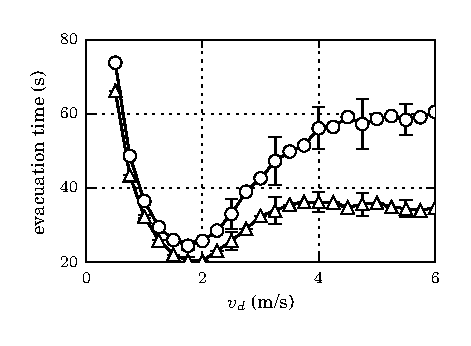
\includegraphics[width=\columnwidth]{./fig1.eps}
\caption{\label{fig:7} Mean evacuation time for 160 individuals (seconds) 
vs. the pedestrian's desired velocity (m/s). The room was $20\times20\,$m 
size. Two contiguous doors were placed on one side of the room as shown in 
Fig.~\ref{fig:19} (see text for details). Mean values were computed from 30 
evacuation processes. Each door was $d_w=1.2$~m width. The desired velocity 
was $v_d=4\,$m/s. Two situations are shown:  $\bigtriangleup$ corresponds to 
the null separation distance between doors, meaning a single door of $2d_w$ 
width. $\bigcirc$ corresponds to the 1~m separation distance between doors  
($d_g=1$~m).   }
% done with fig7_version0.py 
\end{figure}


The evacuation time for separated doors in Fig.~\ref{fig:7} is always above the 
time required to evacuate the pedestrians through the single opening 
(\emph{i.e.} null separation). For $v_d=6\,$m/s, the single opening improves 
the evacuation performance in half of the time that demands the $d_g=1\,$m 
separation configuration. Other separation distances (not shown) exhibit the 
same qualitative pattern as the example presented in Fig.~\ref{fig:7}. 
Therefore, it is clear that while the total width of the opening 
remains unchanged, splitting this width into to symmetric exits affects 
significantly the evacuation performance. \\

We made further research on the $d_g=0$ and $d_g>0$ scenarios. The 
former is investigated in Section \ref{single_double}, while the latter is left 
to Section \ref{door_seperation}. \\

\subsection{\label{single_double}The single door vs. the null separation}

Recall that the $d_g=0$ scenario corresponds to a single opening, but the total 
width of the opening is twice the width of a single door (see 
Section~\ref{faster_is_slower}). Actually, it resembles the situation of a 
double sheet door.  \\

\subsubsection{\label{null_gap_data}The stop-and-go process}

Fig.~\ref{fig:8and9} illustrates on how the evacuation performance improves as 
the opening becomes wider.  Fig.~\ref{fig:9} corresponds to the single door 
($d_w=1.2\,$m), while  Fig.~\ref{fig:8} corresponds to a wider opening 
($3d_w=3.6\,$m), resembling a multi-leaf opening. Both figures represent 
the time evolution of a single pedestrian during an evacuation process. We can 
see the (normalized) pressure acting on the pedestrian and his (her) 
corresponding velocity. The starting point of the pedestrian was 
$(x,y)=(12.35\,\mathrm{m},8.45\,\mathrm{m})$. Notice that an increase in the 
opening width from $d_w$ to $3d_w$ (Fig.~\ref{fig:9} and Fig.~\ref{fig:8}, 
respectively) reduces the evacuation time by one-fifth approximately. \\

\begin{figure*}[!htbp]
\subfloat[Opening of $d_w=1.2$~m width.\label{fig:9}]{
\includegraphics[width=0.75\columnwidth]{./fig2.eps}
% done with fig9_version0.py 
}\hfill
\subfloat[Opening of $3d_w=3.6$~m width. \label{fig:8}]{
\includegraphics[width=0.75\columnwidth]{./fig3.eps}
% done with fig8_version0.py 
}
\caption{\label{fig:8and9} Normalized pressure and velocity on a single 
pedestrian during an evacuation process. Data was recorded from the 
the initial position at $x=12.35$~m and $y=8.45$~m, until the individual left 
the room ($x>20$~m).  The pedestrians desired velocity was $v_d=4\,$m/s. Two 
situations are shown: (a) evacuation through a single door of width 
$d_w=1.2$~m. (b) evacuation through an opening of $3d_w=3.6$~m.} 
\end{figure*}


The pedestrian represented in Fig.~\ref{fig:8and9} increases his (her) 
velocity towards an asymptotic value at the beginning of the processes. This 
value corresponds to the desired velocity $v_d=4\,$m/s. But close to $t=2\,$s, 
the pedestrian suddenly stops because of the clogging around the exit. Clogging 
is also responsible for the pressure increase, as shown in both Fig.~\ref{fig:9} 
and Fig.~\ref{fig:8}. This can be checked over by means of Eq.~(\ref{eqn_2}) 
because when the velocity of the pedestrian vanishes, the desire force 
$\mathbf{f}_d$ attains a maximum (in panic situations only). Notice, however, 
that any further fluctuation of the pressure acting on the pedestrian 
corresponds to an inverse fluctuation on the velocity. Thus, the pedestrian is 
able to reach the exit following a stop-and-go 
process. \\

The instantaneous pressure acting on a single pedestrian can be computed from 
Eq.~(\ref{eqn_4b}) for a slow moving pedestrian (that is, $p_i\simeq 0$). 
The maximum pressure values $\mathrm{P}_\mathrm{max}$ in 
Fig.~\ref{fig:9} and Fig.~\ref{fig:8} are 8550~N.m$^{-1}$ and 6475 N.m$^{-1}$, respectively. 
The corresponding mean pressure values (after the first $2\,$s) are 80\% and 
55\% of the respective maximum values. This means that the mean pressure value for the 
$3d_w$ situation is lower than the corresponding mean value for the $d_w$ situation. 
% This statment is restricted to pedestrians that evacuate through the middle of the room.
That is, the wider opening seems to release pressure from time to time. Consequently, 
the stop-and-go processes are somehow different for the 
single door with respect to the $d_g=0$ situation (the wider opening). \\

{\color{red} The above analyses corresponds to a single pedestrian moving along the middle of 
the room. It does not hold for the whole crowd. For details on the pressure patterns of the 
crowd, see Section \ref{null_gap_patterns}. } 

\subsubsection{\label{null_gap_patterns}The pressure and stream patterns}

For a better understanding on how the pedestrians are (intermittently) released 
from high pressures in the wide opening situation, we pictured the whole scene 
into a pressure contour map and a mean stream path map for all the individuals. 
Fig.~\ref{fig:3} shows the pressure levels ($P_i$) for the 
clogging area. The warm colors are associated to high pressure values. These 
values are close to the corresponding maximum pressure values (not shown). Thus, 
the warm regions define the places where the pedestrians slow down most of the 
time. They are expected to get released only for short periods of time. On the 
contrary, the regions represented in cold colors (low mean pressure) are those 
where the individuals are able to get released for longer time periods. \\

Fig.~\ref{fig:5} represents the mean stream lines during the evacuation 
process. It completes the stop-and-go picture since it exhibits the 
released paths for leaving the room. Notice that the stream lines pass 
through the low pressure regions. That is, it can be seen in Fig.~\ref{fig:5} 
that the stream lines gather along the middle of the clogging area, 
where ``cold'' pressure colors can be found (cf. Fig.~\ref{fig:3}). The 
``warm'' pressure colors are placed on the sides of this region.    \\ 

%%%%%% Vieja "figura 4" (version PDF) %%%%%%%%

%\begin{figure*}[!htbp]
%\subfloat[Mean pressure contour lines (N.m$^{-1}$ units). Colors in the on-line version only.\label{fig:3}]
%{\includegraphics[width=0.75\columnwidth]{./fig4.eps}
% done with fig3_version0.py
%}\hfill
%\subfloat[Mean stream lines. The lines connect the normalized velocity field ($v/v_\mathrm{max}$). The arrows indicate the stream direction.\label{fig:5}]{
%\includegraphics[width=0.75\columnwidth]{./fig5.eps}
% done with fig5_version0.py
%}
%\caption{\label{fig:3and5}Mean pressure and stream lines computed from 30 evacuation processes until 100 pedestrians left the room ($20\,\mathrm{m}\times20\,\mathrm{m}$ size). Data was recorded on a square grid of $1\,\mathrm{m}\times1\,\mathrm{m}$ and then splined to get smooth curves. The red lines at $x=20$~m represent the walls on the right of the room. There is only one opening of $3d_w=3.6$~m width (null separation distance between doors of width $3d_w/2$). The pedestrian's desired velocity was $v_d=4\,$m/s.}
%\end{figure*}

%%%%%%%%%%%%%%%%%%%%%%%%%%%


%%%%%%%%%%% Flow figures %%%%%%%%%%%%%%%%%%%%%

\begin{center}
\CT
\subfloat[Opening of $d_w=1.2$~m width.]{\includegraphics[width=0.75\columnwidth]{./flujo1_2_papercor.eps}}\quad
\subfloat[Opening of $2d_w=2.4$~m width.]{\includegraphics[width=0.75\columnwidth]{./flujo2_4_papercor.eps}}

\subfloat[Opening of $3d_w=3.6$~m width.]{\includegraphics[width=0.75\columnwidth\label{fig:5}]{./fig5.eps}}\quad
\captionof{figure}{Mean stream lines computed from 30 
evacuation processes until 100 pedestrians left the room 
($20\,\mathrm{m}\times20\,\mathrm{m}$ size). The lines connect the normalized velocity field ($v/v_\mathrm{max}$). The arrows indicate the stream direction. Data was recorded on a square grid 
of $1\,\mathrm{m}\times1\,\mathrm{m}$ and then splined to get smooth curves. 
The red lines at $x=20$~m represent the walls on the right of the room. 
The pedestrian's desired velocity was $v_d=4\,$m/s for all the cases.}

\end{center}

%%%%%%%%%%%%%%%%%%%%%%%%%%%%%






We checked over the trajectory of the single pedestrian represented in 
Fig.~\ref{fig:8} and we observed that he (she) managed to get out of the room 
through the path where the stream lines get denser. Thus, Fig.~\ref{fig:8} 
resembles the stop-and-go process for the pedestrians passing through the 
middle of the clogging area, that is, along the low pressure (middle)
region. The pedestrians on the sides of this region (high pressure region) are 
expected to slow down since Fig.~\ref{fig:5} shows no stream lines to the exit. 
\\

Recalling the results in Fig.~\ref{fig:9} for the same single individual as in 
Fig.~\ref{fig:8}, we realize that the single door scene is likely 
to differ from the $d_g=0$ situation since both patterns (for the same 
individual) do. Thus, we examined the pressure contour map for the single door 
and for an opening of twice the single door width. The results are shown in 
Fig.~\ref{fig:2and4}. Fig.~\ref{fig:2} exhibits a similar pressure map pattern 
as Fig.~\ref{fig:3}, but the single door pressure map in Fig.~\ref{fig:4} does 
not. For the single door situation, we do not observe the lower pressure 
pathway in the middle of the clogging area. Instead, high pressure 
is acting on the pedestrians, as shown in the (normalized) pressure evolution 
in Fig.~\ref{fig:9}. The corresponding velocity evolution (Fig.~\ref{fig:9}) 
informs that the pedestrians in this region experience a slow down. \\

%%%%%%%%%%%%%%%% Pressure figures %%%%%%%%%%%%%%%%%%

\begin{center}
\CT
\subfloat[Opening of $d_w=1.2$~m width.\label{fig:4}]{\includegraphics[width=0.75\columnwidth]{./fig6.eps}}\quad
\subfloat[Opening of $2d_w=2.4$~m width. \label{fig:2}]{\includegraphics[width=0.75\columnwidth]{./fig7.eps}}

\subfloat[Opening of $3d_w=3.6$~m width. \label{fig:3}]{\includegraphics[width=0.75\columnwidth]{./fig4.eps}}\quad
\captionof{figure}{\label{fig:2and4} Mean pressure contour lines computed from 30 evacuation processes until 100 pedestrians left the room ($20\,\mathrm{m}\times20\,\mathrm{m}$ size). The scale bar on the right is 
expressed in N.m$^{-1}$ units (see text for details). The red lines at $x=20$~m represent the walls on the right of the room. The pedestrian's desired velocity was $v_d=4\,$m/s. The contour lines were computed on a square grid of $1\,\mathrm{m}\times1\,\mathrm{m}$ and then splined to get smooth curves. Level colors can be seen in the on-line version only.}

\end{center}

{\color{red} Notice, once again, that the results shown in Figs.~\ref{fig:8and9} only resembles the 
situation in the middle of the room. Figs~\ref{fig:5} and Figs.~\ref{fig:2and4} exhibit 
the situation for the whole crowd. However, the mid path in ``cold" colors in~\ref{fig:3} is
the most meaningful region to our research, since it completes the picture
for the stop-and-go process, firstly evidenced in Fig.~\ref{fig:8}.
}


%%%%%%%%%%%%%%%%%%%%%%%%%%%%%%%%%%

At this stage of the investigation we are able to point out a few conclusions. 
The widening of the single door increases the pedestrian's flux, as asserted in 
Ref.~\cite{daoliang1}. In the narrow situation (see Fig.~\ref{fig:9}), 
the pedestrians experience a slow down. The corresponding time delays have been 
associated to blocking structures (see Refs.~\cite{Dorso1,Dorso2}) and causes 
the pressure acting on the nearby individuals to rise. Fig.~\ref{fig:4} 
resembles this situation. However, as the opening widens (\emph{i.e.} the null 
separation situation), the pressure pattern changes qualitatively (see 
Fig.~\ref{fig:3} and Fig.~\ref{fig:2}), allowing the pedestrians in the middle 
of the clogging area to make a pathway to the exit. This pathway corresponds to 
the breaking of the blocking structures.   \\

\subsection{\label{door_seperation} Separated doors}

We will now analyze the case in which the evacuation process is through two 
doors, symmetrically placed on the same side of the room. We will explore the 
dependence of such a process on the doors separations. We will assume that 
each door width is $d_w=1.2\,$m.  \\

It has been shown in Fig.~\ref{fig:7} that separating the doors a distance 
$d_g=1\,$m worsens the evacuation performance with respect to the null 
separation. We  further explored this worsening by increasing $d_g$ at steps of 
$0.5\,$m, starting from the null separation distance. Fig.~\ref{fig:13} shows 
the mean evacuation time and the corresponding error bars (indicating the 
$\pm\sigma$ limits). The desired velocity was set to $v_d=4\,$m/s, where the 
``faster is slower'' effect takes place. \\

\begin{figure}
\includegraphics[width=\columnwidth]{./fig8.eps}
\caption{\label{fig:13} Mean evacuation time for 225 pedestrians (room of 
$20\times20$~m size) as a function of the doors separation distance. Mean 
values were computed from 30 evacuation processes until 160 pedestrians left 
the room. Each door was $d_w=1.2$~m width for non-vanishing gaps. The null gap 
means a single door of $2d_w$ width. The desired velocity was $v_d=4\,$m/s. }
% done with fig13_version0.py 
\end{figure}

The evacuation time as a function of $d_g$ shown in Fig.~\ref{fig:13} is one 
of our main results. The worsening in the evacuation performance rises to a 
maximum value at $1\,$m while its slope changes sign for $d_g>1\,$m. Thus, 
$d_g=1\,$m appears to be the worst evacuation scenario for the 
$20\,\mathrm{m}\times20\,\mathrm{m}$ room with 225 individuals and two 
doors of $d_w=1.2\,$m each (see Fig.~\ref{fig:13}).  \\


We further computed the mean evacuation time for an increasing number of 
pedestrians (and room sizes). We kept the pedestrian density unchanged (at 
$t=0$) for all the simulation processes. Fig.~\ref{fig:1} exhibits the mean 
evacuation time per pedestrian as a function of the separation distance 
(\emph{i.e.} gap). We divided the evacuation time by the total number of 
pedestrians for visualization reasons. \\


\begin{figure}
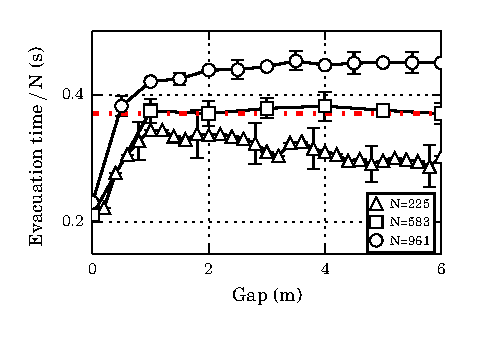
\includegraphics[width=\columnwidth]{./fig9.eps}
\caption{\label{fig:1} Mean evacuation time per total number of pedestrians 
that left the room ($N$), as a function of the doors separation distance. Mean 
values were computed from 30 evacuation processes. Each door was $d_w=1.2$~m 
width for non-vanishing gaps. The null gap means a single door of $2d_w$ width. 
Three situations are shown: $\bigtriangleup$ corresponds to the $20\times20$~m 
room when 160 pedestrians left the room, $\Box$ corresponds to $30\times30$~m 
room when 530 pedestrians left the room, and $\bigcirc$ corresponds to 
$40\times40$~m room when  865 pedestrians left the room.  {\color{red} The red (online version only) dashed line represents half the evacuation time for 225 individuals in a room with a single door of $d_w=1.2$~m. The desired velocity  was $v_d=4\,$m/s. for all cases.}}
% done with fig1_version0.py 
\end{figure}

The results shown in Fig.~\ref{fig:1} were not expected. The evacuation time 
settles to an asymptotic value for separation distances $d_g>5\,$m. The mean 
evacuation time becomes almost independent of the separation distances $d_g$ 
despite that the clogging areas around the doors might still overlap.  \\ 

{\color{red} Fig.~\ref{fig:1} includes (half) the  evacuation time for the 20$~\times$~20 room with a single exit (see caption for details). Notice that the asymptotic limit for the evacuation time (when two doors are separated 6~m) does not match exactly the single exit situation. This fact corresponds to the difference in the bulk pressures on each case. That is, the bulk pressure for the single door situation is expected to be higher than the one for the two doors situation (and a 6~m gap) because of the difference in the number of individuals pushing towards each door. Thus, the evacuation time worsens for the single door situation.}\\

Fig.~\ref{fig:1} also shows that the slope not always changes sign  
at $d_g\simeq1\,$m. Furthermore, as the number of pedestrians is increased for 
$d_g>1\,$m, the evacuation time slope raises to positive values. The 
greater the number of pedestrians, the worst the evacuation time (per 
individual). This appears to occur for $d_g>1\,$m, regardless of the crowd 
size. That is, according to Fig.~\ref{fig:1}, there exists a separation 
distance value $d_g\simeq1\,$m where the evacuation slope changes sharply 
to negative or positive values (for $d_g>1\,$m). This phenomenon has not been 
studied in the literature, to our knowledge. \\

We can resume the results in Fig.~\ref{fig:1} in the following way: the 
evacuation time rises when the doors separation increases from a wide opening 
(null separation distance) to the distance $d_g\simeq1\,$m. At this gap, the 
evacuation time slope changes notably, entering a much slowly 
varying regime towards an asymptotic value (for $d_g\gg1\,$m).  The former can 
be identified as a regime for small values of $d_g$, while the latter is valid 
for moderate to large values of $d_g$. The fact that a sharp change occurs at 
$d_g\simeq1\,$m, no matter the crowd size, suggests that both regimes are 
somehow different in nature. This moved us to explore the two regimes 
separately. \\

\subsubsection{\label{small_regime} The regime for $d_g<1\,$m}

Our starting point is the pressure contour map, since we can easily compare the 
current patterns with those presented in Section~\ref{null_gap_patterns}. 
Fig.~\ref{fig:16} shows the mean pressure pattern for the separation distance 
$d_g=1.5\,$m, that is, close to the gap value where the sharp change in the 
slope occurs. The differences between Fig.~\ref{fig:16} and 
Fig.~\ref{fig:2and4} are noticeable. We can now see a wide region in the center of 
the clogging area representing the high pressure ($P_i$) acting 
on each pedestrian (warm colors in Fig.~\ref{fig:16}). The regularity in the 
colors of this region is meaningful: the high pressure acting on the pedestrians 
does not allow a regular stream (pathway) to the exit. This is in agreement with 
the evacuation time worsening shown in Fig.~\ref{fig:13}.   \\

{\color{red} In all cases the pressure maps showed a resemblance with the ones reported in Ref.~\cite{Zhang}}\\

\begin{figure*}[!htbp]
\subfloat[Separation distance of $d_g=1.5$~m.\label{fig:16}]{
\includegraphics[width=0.75\columnwidth]{./fig10.eps}
% done with fig16_version0.py 
}\hfill
\subfloat[Separation distance of $d_g=5$~m. \label{fig:17}]{
\includegraphics[width=0.75\columnwidth]{./fig11.eps}
% done with fig17_version0.py 
}
\caption{\label{fig:16and17} Mean pressure contour lines computed from 30 
evacuation processes until 100 pedestrians left the room 
($20\,\mathrm{m}\times20\,\mathrm{m}$ size). The scale bar on the right is 
expressed in N.m$^{-1}$ units (see text for details). The red lines at 
$x=20$~m represent the walls on the right of the room. The pedestrian's desired 
velocity was $v_d=4\,$m/s. The contour lines were computed on a square grid of 
$1\,\mathrm{m}\times1\,\mathrm{m}$ and then splined to get smooth curves. Level 
colors can be seen in the on-line version only.} 
\end{figure*}


Fig.~\ref{fig:16} suggests that blocking structures might be present for long 
time periods, since the pedestrians cannot manage to get out easily. We 
examined this possibility through the \textit{blocking probability}. In this 
context, the blocking probability is associated to the ratio between the time 
that each door remains blocked with respect to the total evacuation time (cf. 
Section~\ref{human}). Fig.~\ref{fig:14} presents two kinds of blockings: the 
simultaneous blocking of both doors, and the blocking of a single door (say, 
the one on the left). The former connects the left most wall with the right 
most wall, but does not contact the separation wall in the middle of the walls. 
The latter connects the walls on both sides of the selected door (say, 
the one on the left). \\


\begin{figure}
\includegraphics[width=\columnwidth]{./fig12.eps}
\caption{\label{fig:14} Ratio between time steps including blocking structures 
and the total number of time steps for 30 evacuation processes, as a function 
of the doors separation distance. The room size was $20\times20$~m with 225 
occupants. Each door was $d_w=1.2$~m width for non-vanishing gaps. The null gap 
means a single door of $2d_w$ width. The desired velocity was $v_d=4\,$m/s.  
$\bigcirc$ corresponds blocking structures connecting both the left side wall 
of the left door with the right side wall of the right door (see text for 
details). $\Box$ corresponds to blocking structures connecting both sides of a 
single door (see text for details).   }
% done with fig14_version0.py 
\end{figure}

According to Fig.~\ref{fig:14}, the single door blockings are not relevant 
until $d_g\simeq1\,$m, while the simultaneous blockings weaken as the gap 
(separation distance $d_g$) increases. The single door blockings resemble the 
response in Fig.~\ref{fig:13}, and thus, we conclude that this kind of 
blockings should play an important role in the increase of the evacuation time 
for small gaps $d_g$. Notice that single door blocking probability explains the 
75\% of the evacuation time, as can be seen in Fig.~\ref{fig:14}. \\

The results so far moved us to focus closer on the dynamics around each door. 
We watched many animations of the evacuation process for gap distances between 
the null separation to $d_g=1.5\,$m (not shown). We realized that single 
door blockings hold if the gap is large enough to accommodate at least two 
pedestrians. That is, any blocking structure enclosing a single door can hold 
for some time if the pedestrians at the end of the structure (and in contact 
with the walls) do hardly leave the structure. Two pedestrians are needed at the 
gap wall to ensure that both doors remain blocked.\\ 

We want to call the attention on the fact that when $d_g$ passes through the 
$1\,$m situation, the kind of simultaneous blocking without contacting the gap 
wall, is replaced by the kind of single door blockings acting (usually) 
simultaneously. This achieves a qualitative different pressure and 
stream pattern. As shown in Fig.~\ref{fig:2}, the widening of the exit 
allows a pathway through the middle of the clogging area. This is likely to 
occur even for very small gaps (see Fig.~\ref{fig:14}). However, the single door 
blockings follow a pressure pattern similar to  Fig.~\ref{fig:4} on each door.  
What we see in Fig.~\ref{fig:16} is the combined pattern built from two 
single door patterns as in Fig.~\ref{fig:4}. \\

We conclude from the analysis of small gaps ($d_g<1\,$m) that a door 
separation distance roughly equal to two pedestrian widths is critical. 
This distance allows persistent single door blockings. Small distances (close 
to the null separation) do not actually allow single door blockings to hold for 
long time. Thus, the role of $d_g=2r_{ij}$ (two pedestrian's width) is decisive to move the evacuation 
process from one regime to another. \\ 


\subsubsection{\label{large_regime} The regime for $d_g>1\,$m}

Fig.~\ref{fig:14} shows that the single door blockings (see 
 Section~\ref{small_regime}) remains around 75\% of the total evacuation time 
for $d_g>1\,$m (225 individuals in the room). We also computed this magnitude 
for situations with increasing number of individuals (see Fig.~\ref{fig:15}). 
The probability of single door blockings approaches unity as the crowd size 
increases. This means, according to our definition of blocking probability, 
that the blocking time raises as the number of individuals increases. The gap 
distance, however, does not play a significant role for $d_g>1\,$m.  \\ 


\begin{figure}
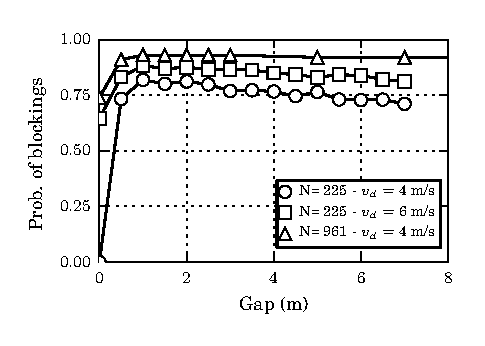
\includegraphics[width=\columnwidth]{./fig13.eps}
\caption{\label{fig:15} Ratio between time steps including blocking structures 
and the total number of time steps for 30 evacuation processes, as a function 
of the doors separation distance. The only blocking structures considered 
were those connecting both sides of one single door (see text for details). 
Each door was $d_w=1.2$~m width for non-vanishing gaps. The null gap means a 
single door of $2d_w$ width. Three scenarios are shown: $\bigcirc$ 
corresponds to the room of size $20\times20$~m with 225 occupants and a 
desired velocity of $v_d=4\,$m/s. $\Box$ corresponds to the room of size  
$20\times20$~m with 225 occupants and a desired velocity of $v_d=6\,$m/s. 
$\bigtriangleup$ corresponds to the room of size $40\times40$~m with 961 
occupants and a desired velocity of $v_d=4\,$m/s.   }
% done with fig15_version0.py 
\end{figure}

There is a noticeable difference between the evacuation time 
shown in Fig.~\ref{fig:1} and the blocking probability exhibited in 
Fig.~\ref{fig:15}. Fig.~\ref{fig:1} presents the evacuation time for three 
different room sizes and increasing number of pedestrians.  The slope of the 
evacuation curve is negative for the $20\times20\,$m room, it vanishes for 
the $30\times30\,$m situation and it becomes slightly positive for the 
$40\times40\,$m room (for $d_g>1\,$m). Thus, as the number of pedestrians 
increases, the slope of the evacuation time changes sign. However, this does not 
occur for the blocking probability (see Fig.~\ref{fig:15}). The slope of the 
blocking probability remains always negative for an increasing number of 
pedestrians (and desire velocities). Therefore, the changes in the slope 
observed in Fig.~\ref{fig:1} cannot be explained by changes in the blocking 
time (\textit{i.e} blocking probability).   \\

We checked the pressure patterns for $d_g>4d_w$ (see Fig.~\ref{fig:17} as an 
example). We came to the conclusion that since the evacuation slope in 
Fig.~\ref{fig:1} changes with an increasing number of individuals, the whole 
bulk should be involved in this phenomenon. Therefore, we focused our 
investigation on the pressure contribution of the whole bulk.  \\ 

As shown in Eq.~(\ref{eqn_5}) of \ref{alternative} , we can realize that the pressure of the 
whole bulk (left-hand side) is related to the total desire force contribution 
(right-hand side). Thus, the pressure of the bulk can vary in two possible 
ways: if the desire force of the individuals (\emph{i.e.} anxiety levels) 
changes, or, if the crowd size changes. An increase on either 
the number of evacuating pedestrians ($N$) or their corresponding anxiety 
level ($v_d$), will increase the pressure of the whole bulk. {\color{red} This result is in accordance with the experiment performed in Ref.~\cite{Pastor}.}
A simple example is presented in the Appendix. \\

Fig.~\ref{fig:1} exhibits the evacuation time for an increasing number of 
pedestrians. But, an increase in the pedestrians anxiety level should  
resemble similar results, if the above reasonings are true. Fig.~\ref{fig:12} 
shows the evacuation time as a function of the separation distance for two 
different desired velocities. As expected, the sharp change in the slope occurs 
around $d_g=2r_{ij}$. Also the slope changes as the desired velocity ($v_d$) is 
increased (\emph{i.e.} higher anxiety level). This confirms that the social 
pressure is responsible the slope behaviour shown in Fig.~\ref{fig:1}. \\

{\color{red} Notice that Fig.~\ref{fig:12} exhibits a crossover for a gap of 0.5~m. This crossover is related to the slightly negative slope shown in Fig.~\ref{fig:7}. We want to stress the fact that this crossover appears for desired velocities between 6~m/s and 8~m/s (see  Fig~\ref{fig:7}), but not for increasing number of pedestrians at lower desired velocities (see Fig.~\ref{fig:15}). Despite the fact that we are able to see a crossover in the range of 6~m/s to 8~m/s, we prevent the reader that not noticeable consequences were found that could affect further conclusions, since the ``faster is slower'' effect remains valid within the sudied range.  }


\begin{figure}
\includegraphics[width=\columnwidth]{./fig14.eps}
\caption{\label{fig:12} Mean evacuation time for 225 pedestrians (room of 
$20\times20$~m size) as a function of the doors separation distance. Mean 
values were computed from 30 evacuation processes until 160 pedestrians left 
the room. Each door was $d_w=1.2$~m width for non-vanishing gaps. The null gap 
means a single door of $2d_w$ width. $\bigcirc$ corresponds to pedestrians 
with desired velocity of $v_d=4\,$m/s. $\Box$ corresponds to pedestrians 
with desired velocity of $v_d=8\,$m/s. }
% done with fig12_version0.py 
\end{figure}


We conclude from the analysis of large gaps ($d_g>1\,$m) that the evacuation 
time is controlled by the social pressure in the bulk. The crowd size and 
the desired velocity $v_d$ affects the pressure acting on the pedestrians. 
For $d_g>5\,$m in our simulations, the evacuation time is very close to the 
corresponding asymptotic value, although the bulks around each door are not 
completely independent. This means that the mixing of both crowds (that is, 
the fact that the bulks are in contact) do not affect strongly the evacuation 
performance.   \\







\section{\label{conclusions}Conclusions}


We examined in detail the evacuation of pedestrians for the situation where 
two contiguous doors are available for leaving the room. Throughout  
Section~\ref{results} we presented results on the evacuation performance under 
high anxiety levels and increasing number of pedestrians. Both conditions 
exhibit the novel result that a worsening in the evacuation time exists as the door 
separation distance $d_g$ increases from the null value to roughly the width of 
two pedestrians. Special situations may enhance the evacuation performance for 
larger values of $d_g$. \\

The range from $d_g=0$ to $d_g\gg d_w$ was inspected. 
In the interval $0\leq d_g \leq 2r_{ij}$ (two pedestrian's width), the evacuation 
performance worsened for all the explored situations, as the separation
distance between doors $d_g$ increased. But, from $d_g > 2r_{ij}$ the 
evacuation time enhanced for relatively small crowds and moderate anxiety
levels. We realized that the sharp change in the evacuation behaviour at
$d_g=2r_{ij}$ corresponded to qualitative differences in 
the pedestrian dynamics close to the exits.\\

After a detailed comparison of the dynamics for the single door situation and 
for two doors very close to each other (that is, $d_g<2r_{ij}$), we concluded that 
the blocking structures (\emph{i.e.} blocking arcs) around the openings were 
released intermittently, allowing the pedestrians to leave the room in a 
stop-and-go process. As the separation distance approached $2r_{ij}$, the 
blocking arcs around each door, resembled the blocking 
situation of two single doors. This changes only affected the 
local dynamics (close to the doors), while the crowd remained gathered into a 
single clogging area. \\

For $d_g>2r_{ij}$ the single door blocking structures become relevant even for 
large values of $d_g$ (see Fig.~\ref{fig:14}). No further qualitative changes 
were observed locally around each door. However, increasing the crowd size ($N$) 
or the pedestrian's anxiety level ($v_d$) slowed down the evacuation. Both 
magnitudes are linked to the pressure acting on the pedestrians, and therefore, 
enhanced the ``faster is slower'' effects. \\

For a better understanding of the relationship between $N$, $v_d$ and the 
pressure in the bulk, a simple lane example complemented our analysis. It was 
shown that the classical virial expression is still suitable for the 
investigation of social systems.  \\




\section{\label{acknowledgments}Acknowledgments}

C.O.~Dorso is a main researcher of the National Scientific and Technical 
Research Council (spanish: Consejo Nacional de Investigaciones Cient\'\i ficas y 
T\'ecnicas - CONICET), Argentina. G.A.~Frank is an assistant researcher of the 
CONICET, Argentina. I.M.~Sticco and S.~Cerrotta have degree in Physics.


\appendix


\section{\label{alternative}Alternative definition for the social pressure}

Recall that the social force model (SFM) deals with the pedestrians desire and 
their private space preservation. Although the desire force 
$\mathbf{f}_d$ is a ``unilateral'' force, the Newton equations of 
motion remain valid. Therefore, it can be derived from the virial relation 
that \cite{lion}

\begin{equation}
 \bigg\langle\displaystyle\sum_{i=1}^N\displaystyle\frac{p_i^2}{m_i} + 
\displaystyle\sum_{i=1}^N 
\mathbf{r}_i\cdot\mathbf{f}_i\bigg\rangle=-2\mathcal{PA}\label{eqn_3}
\end{equation}


\noindent for the set of $N$ pedestrians inside an area $\mathcal{A}$. $p_i$  
and $\mathbf{f}_i$ are the momentum and total force acting on the individual 
$i$ 
(excluding the interaction with the walls). $\langle\cdot\rangle$ corresponds 
to 
the mean value along time. The right hand side $-2\mathcal{PA}$ defines the 
global pressure on the curve enclosing the surface $\mathcal{A}$.  \\

Following Ref.~\cite{lion} we can define the ``social pressure function'' $P_i$ 
as\\

\begin{equation}
2P_i\mathcal{A}_i=\displaystyle\frac{p_i^2}{m_i} + \frac{1}{2}
\displaystyle\sum_{j=1}^{N-1}
\mathbf{r}_{ij}\cdot\mathbf{f}_s^{(ij)}\label{eqn_4}
\end{equation}

\noindent where $\mathcal{A}_i$ is the area enclosing the pedestrian $i$ and 
$\mathbf{r}_{ij}=\mathbf{r}_{i}-\mathbf{r}_j$. Notice that the inner product 
$\mathbf{r}_{ij}\cdot\mathbf{f}_s^{(ij)}$ is always positive for repulsive 
feelings.  \\ 

The ``social pressure function'' $P_i$ is roughly similar to the literature 
definition \cite{Helbing1}, as expressed in Eq.~(\ref{eqn_4b}), for neglectable 
momentum $p_i$. Furthermore, Eqs.~(\ref{eqn_4b}) and (\ref{eqn_4}) become 
equal if the area $\mathcal{A}_i$ and $r_{ij}$ are replaced by $\pi r_i^2$ and 
the contacting distance $2r_i$, respectively. \\

We can further compute the pressure on all the pedestrians according to  
Eq.~(\ref{eqn_3}). Notice that the force sum can be split into the summation of 
three contributions:  the desire forces, the social forces and the granular 
forces. Actually, the granular force does not play a role because of 
orthogonality ($\mathbf{r}_{ij}\cdot\mathbf{f}_g^{(ij)}=0$). Consequently, 
replacing Eq.~(\ref{eqn_4}) into the virial relation (\ref{eqn_3}) gives \\  



\begin{equation}
 \displaystyle\sum_{i=1}^N\langle2P_i\mathcal{A}_i 
\rangle=-2\mathcal{PA}-\displaystyle\sum_{i=1}^N \langle
\mathbf{r}_i\cdot\mathbf{f}_d^{(i)}\rangle\label{eqn_5}
\end{equation}


We should remark that Eq.~(\ref{eqn_5}) holds either if the pedestrians are in 
contact or not. The ``social pressure function'' $P_i$ makes possible 
for the individuals to change their behavioural pattern when they come too 
close to each other. \\ 

\section{\label{app}The lane example}

We decided to open this supplementary section in order to make clear the 
meaning of the ``social pressure'' acting on an individual and the collective 
pressure (that is, the \textit{bulk} pressure) on a set of individuals. We 
will follow a simple example as a guide for more general situations. \\

\subsection{\label{social_pressure}The social pressure}

Fig.~\ref{fig:18} represents a lane of individuals pushing to the right. The 
ending wall prevents the individuals from moving. All the pedestrians in the 
lane are at their equilibrium positions $x_1,x_2,...,x_{i},...x_N$, 
while the wall is placed at the position $x_0=0$ (see Fig.~\ref{fig:18}).  \\

\begin{figure}[!htbp]
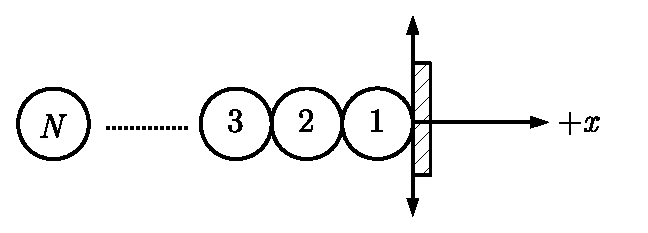
\includegraphics[width=0.75\columnwidth]{./fig15.eps}
\caption{\label{fig:18} Lane of individuals pushing to the right. The 
horizontal axis indicates the positive direction.  }
% done with figuras_presion.odg
\end{figure}

The pedestrians push to the right acknowledging a desired force 
$f_d^{(i)}=mv_d/\tau$, according to Eq.~(\ref{eqn_2}). The social repulsion 
feelings balance this desire force, but only the contacting neighbors are 
relevant to these feelings. Thus, the balance equation for any pedestrian 
in the lane reads \\

\begin{equation}
 f_s^{(i,i+1)}-f_s^{(i,i-1)}+\displaystyle\frac{mv_d}{\tau}=0\label{eqn_6}
\end{equation}

\noindent for $f_s^{(i,j)}$ meaning the repulsive feelings of pedestrian $i$ 
due to the presence of pedestrian $j$. Notice that the boundary condition at 
the wall-end is $x_0=0$ (Dirichlet condition), while the condition at the free 
end is $f_s^{(N,N+1)}=0$ (Neumann condition). The forces on the pedestrians can 
be obtained recursively from Eq.~\ref{eqn_6}, starting at the free ended 
individual ($i=N$). The resulting expression is 

\begin{equation}
f_s^{(i,i-1)}=(N-i+1)\,\displaystyle\frac{mv_d}{\tau}\ \ \ , \ \ \ 
i=1,....,N\label{eqn_7}
\end{equation}

\noindent while the corresponding positions $x_1,x_2,...,x_{i},...x_N$ are 
obtained by a backward substitution of the social forces expressed in 
Eq.~(\ref{eqn_2}), starting at the wall-end

\begin{equation} 
x_i=x_{i-1}-(r_{i}+r_{i-1})+B\,\ln\bigg[(N-i+1)\,\displaystyle\frac{mv_d}{A\tau}
\bigg]\label{eqn_8}
\end{equation}


The pressure on a single pedestrian $P_i$ corresponds to the forces acting on 
him (her) (per unit length) due to the neighboring pedestrians. According to 
Eqs.~(\ref{eqn_4b}), the pressure for any individual $i$ in the lane is  

\begin{equation}
P_i=\displaystyle\frac{1}{2\pi 
r_i}\,\bigg[f_s^ { (i , i+1) } +f_s^{(i,i-1)}\bigg]\label{eqn_10}
\end{equation}

We can also arrive to this expression through the ``social pressure 
function'' definition (\ref{eqn_4}) 

\begin{equation}
P_i=\displaystyle\frac{1}{2}\,\bigg[\displaystyle\frac{x_{i}-x_{i+1}}{
2\mathcal{A}_i } \,
f_s^ { (i , i+1) } +\displaystyle\frac { 
x_{i-1}-x_{i}}{2\mathcal{A}_i}\,f_s^{(i,i-1)}\bigg]\label{eqn_9}
\end{equation}

\vspace{3mm}

\noindent where the magnitude $x_{ij}/2\mathcal{A}_i$ corresponds to the 
(inverse) effective length of the pedestrian. For individuals modeled as 
circles, the inter-pedestrian distance is roughly $x_{ij}=2r_i$ and the area 
is $\mathcal{A}_i=\pi r_i^2$. Thus, both definitions agree. However, the 
last one is preferred since it does not assume that the forces actuate 
exactly at the distance $r_i$, as already mentioned in Section \ref{pressure}. 
\\


\subsection{\label{bulk_pressure}The bulk pressure}

We can now illustrate on how to compute the virial relation (\ref{eqn_5}). We 
can add the social pressures expressed in (\ref{eqn_9}) for the $N$
pedestrians in the lane.


\begin{equation}
\left\{\begin{array}{lcl}
2P_1\mathcal{A}_1 
& = &\displaystyle\frac{x_{1}}{2}f_s^ { (1 , 2)} - 
\displaystyle\frac{x_{2}}{2}\,f_s^ { (1 , 2) }  \\
&& \\
2P_2\mathcal{A}_2 
& = &\displaystyle\frac{x_{2}}{2}\,\big[f_s^ { (2 , 3)} - f_s^{(2,1)} 
\big] - \displaystyle\frac{x_{3}}{2}\,f_s^ { (2 , 3) } +\displaystyle\frac 
{ x_ {1}}{2}\,f_s^{(2,1) 
} \\
&& \\
2P_3\mathcal{A}_3 
& = &\displaystyle\frac{x_{3}}{2}\,\big[f_s^ { (3 , 4)} - f_s^{(3,2)} 
\big] - \displaystyle\frac{x_{4}}{2}\,f_s^ { (3 , 4) } +\displaystyle\frac 
{ x_{2}}{2}\,f_s^{(3,2) 
} \\
... &&\\
&& \\
2P_N\mathcal{A}_N 
& = &-\displaystyle\frac{x_{N}}{2}\, f_s^{(N,N-1)} 
+\displaystyle\frac{ x_{N-1}}{2}\,f_s^{(N,N-1) 
} \\
 \end{array}\right.\label{eqn_11}
\end{equation}

These are the local pressures on each pedestrian due to the 
contacting neighbors (and excluding the wall). Adding the terms results 
in the virial relation, as expressed in (\ref{eqn_5})

\begin{equation}
\begin{array}{lcl}
\displaystyle\sum_{i=1}^N 2P_i\mathcal{A}_i & = & (x_1 - x_2)f_s^{(1,2)} + (x_2 
- 
x_3)f_s^{(2,3)} +... \\
& + &  (x_{N-1}-x_N)f_s^{(N,N-1)} \\
&& \\
& = & x_{1}\,\displaystyle\frac{N\,mv_d}{\tau} - 
\displaystyle\sum_{i=1}^N x_i\,\displaystyle\frac{mv_d}{\tau} \\
 \end{array}\label{eqn_12}
\end{equation}

\noindent where the first term on the right corresponds to the global pressure 
$-2\mathcal{PA}$. Notice that $x_1$ is negative, and thus, $2\mathcal{PA}$ is 
defined as a positive magnitude. The last term is also positive, adding 
pressure to the bulk due to the desire forces.  
\\

The virial relation (\ref{eqn_5}) allows to compute the \textit{bulk} pressure 
on a group of pedestrians. For example, the pressure on the $M$ pedestrians 
closest to the wall corresponds to the force acting on this group due to the 
other $N-M$ pedestrians. According to Eq.~(\ref{eqn_5}), the 
pressure on the $M$ individuals is    


\begin{equation}
 \displaystyle\sum_{i=1}^M 2P_i\mathcal{A}_i 
=-2\mathcal{PA}-\displaystyle\sum_{i=M+1}^N 
2P_i\mathcal{A}_i-\displaystyle\sum_{i=1}^N 
x_i\displaystyle\frac{mv_d}{\tau}\label{eqn_13}
\end{equation}


The \textit{bulk} pressure on the first $M$ individuals increases as more 
individuals are included in the crowd. This can be verified by evaluating 
Eq.~(\ref{eqn_12}) and Eq.~(\ref{eqn_13}) for increasing values of $N$. \\

The Eqs.~(\ref{eqn_7}) and (\ref{eqn_8}) allow to compute the pedestrian 
pressure profile as a function of the distance to the wall. The profile is 
qualitatively similar to the one measured during an evacuation process. 
Fig.~\ref{fig:10} represents the histogram for the pressure on each 
pedestrian, computed as in Eq.~\ref{eqn_4b} and Eq.~\ref{eqn_4} (see caption for
details). \\


\begin{figure}[!htbp]
\includegraphics[width=\columnwidth]{./fig16.eps}
\caption{\label{fig:10} Mean pressure as a function of the distance 
to the exit. The room was $20\,\mathrm{m}\times20\,\mathrm{m}$ size and 
included one door of $d_w=1.2$~m width. Mean values were computed from 30 
evacuation processes, until 100 pedestrians left the room. The desired velocity 
was $v_d=4\,$m/s. The distance to the door was binned into equal intervals of 
$0.3$~m.  The $\bigcirc$  symbols correspond to the mean pressure computed as 
in \ref{eqn_4} for neglectable momentum ($p_i=0$) and $\mathcal{A}_i=\pi 
r_i^2$. The symbols $\bigtriangleup$ correspond to the mean pressure computed as 
in \ref{eqn_4b} (see text for details).  }
% done with fig10_version0.py 
\end{figure}





%% main text
%%\section{}
%%\label{}

%% The Appendices part is started with the command \appendix;
%% appendix sections are then done as normal sections
%% \appendix

%% \section{}
%% \label{}

%% If you have bibdatabase file and want bibtex to generate the
%% bibitems, please use
%%
\bibliographystyle{elsarticle-num} 
\bibliography{paper}

%% else use the following coding to input the bibitems directly in the
%% TeX file.

%%\begin{thebibliography}{00}

%% \bibitem{label}
%% Text of bibliographic item

%%\bibitem{}

%%\end{thebibliography}
\end{document}
\endinput
%%
%% End of file `elsarticle-template-num.tex'.
